% $Id: TimeMgr_desdoc.tex,v 1.1 2002/08/18 22:43:36 eschwab Exp $

\documentclass[]{article}

\usepackage{epsf}
\usepackage{html}
\usepackage[T1]{fontenc}
\usepackage[dvips]{graphics,color}

\textwidth 6.5in
\textheight 8.5in
\addtolength{\oddsidemargin}{-.75in}

\begin{document}

\bodytext{BGCOLOR=white LINK=#083194 VLINK=#21004A}

\begin{titlepage}

\begin{center}
{\Large Earth System Modeling Framework } \\
\vspace{.25in}
{\Large {\bf Time Manager Design}} \\
\vspace{.25in}
{\large {\it Earl Schwab}} \\
\vspace{.25in}
{August 16, 2002}
\vspace{.5in}
\end{center}

\begin{latexonly}
\vspace{5.5in}
\begin{tabular}{p{5in}p{.9in}}
\hrulefill \\
\noindent {\bf NASA Earth Science Technology Office} \\
\noindent Computational Technologies Project \\
\noindent CAN 00-OES-01 \\
\noindent http://www.esmf.ucar.edu \\
\end{tabular}
\end{latexonly}

\end{titlepage}

\tableofcontents

\newpage
\section{Synopsis}
% $Id: TimeMgr_syn.tex,v 1.1 2002/08/18 22:43:36 eschwab Exp $

%\section{Synopsis}

The Earth System Modeling Framework (ESMF) Time Management Library
provides utilities for time and date representation and calculation,
and higher-level utilities that control model time stepping and alarming.
It is designed to meet the requirements as specified in the ESMF Time
Manager Requirements document \cite{timemgr_req}.


\section{Object Model}
% $Id: TimeMgr_obj1.tex,v 1.4 2003/08/12 14:32:50 cdeluca Exp $

\subsection{Object Model}

The core Time Manager Library consists of six object-oriented classes (types)
organized in four layers of inheritance, aggregation and composition,
as shown in Figure 1 below.  The primary classes intended for
direct model use are:

\begin{itemize}
\item {\tt ESMF\_TimeInterval}
\item {\tt ESMF\_Time}
\item {\tt ESMF\_Clock}
\item {\tt ESMF\_Alarm}
\item {\tt ESMF\_Calendar}
\end{itemize}

These directly correspond to, and encapsulate the representation and
behavior of, Time Intervals, Time instants, Clocks, Alarms, and Calendars,
as specified in the ESMF Time Manager Requirements document.
{\tt ESMF\_TimeInterval} is independent of any calendar (except when used
as a Calendar interval), whereas {\tt ESMF\_Time} is dependent on a calendar
type, such as Gregorian or Julian.  Multiple objects of all these primary
classes can be instantiated within a single application.

There is also one secondary supporting class, not intended for direct
use in model applications.  This is {\tt ESMF\_BaseTime}.  {\tt ESMF\_BaseTime}
serves as the base class for both {\tt ESMF\_TimeInterval} and
{\tt ESMF\_Time},capturing common core time representation and functionality.

{\tt ESMF\_Calendar} encapsulates all the required calendar types and behavior,
isolating them from Time instants.  Specific calendar-type objects (e.g.
Gregorian, Julian, no-leap, etc.) can be instantiated from {\tt ESMF\_Calendar}.
Ideally, for a given application, no more than one calendar
object should be instantiated for each calendar type.  The idea is that
a calendar object is analogous to a "wall calendar," serving as a single
point of reference throughout an application.  For example, a single
Gregorian calendar can be instantiated within an application and shared
among all the time instants.  However, the design does not preclude having
multiple calendar instantiations.  For practical reasons of using SPMD or
MPMD application execution models, there may be multiple instantiations
of a calendar type; for example, one per component.

For object integrity, all class data members are private; access is via
public member functions only. The entire {\tt ESMF\_BaseTime} base class
will be "protected," so that it can only be inherited; it will not be directly
instantiable.

\begin{center}
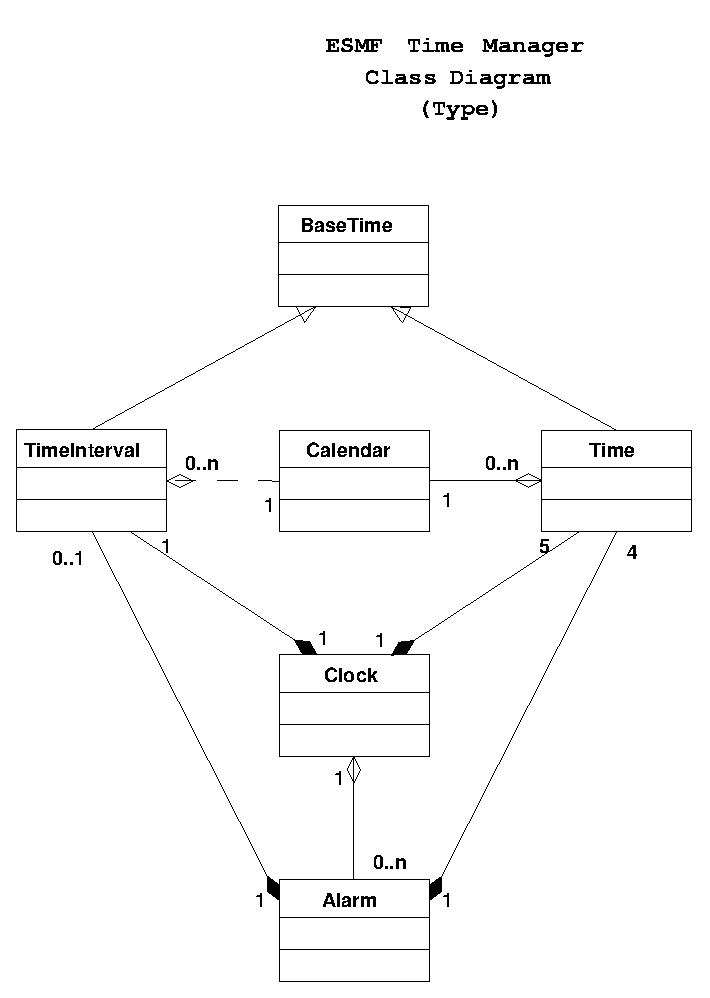
\includegraphics{TimeMgrClass.EPS}
   
Figure 1.  ESMF Time Manager Class Diagram
   
\end{center}

% $Id: TimeMgr_obj2.tex,v 1.1 2002/08/18 22:43:36 eschwab Exp $

%\section{Object Model}

Figure 2 shows the typical usage (instantiantion) of the Time Manager
within an application.  First, a calendar is created.  Then, time intervals
and time instants are created for clock usage and initialized as a time step,
start time, stop time and current time.  Similarly, a time interval and time 
instants are created and initialized for alarm usage.  Next, alarms are
created and intialized with the appropriate previously created time interval
and time instants.  Finally, a clock is created and initialized with its
corresponding time instants and time interval.  The clock is also associated
with the previously created calendar and alarms.  The clock is then ready
for timestepping and alarm checking.

\begin{center}
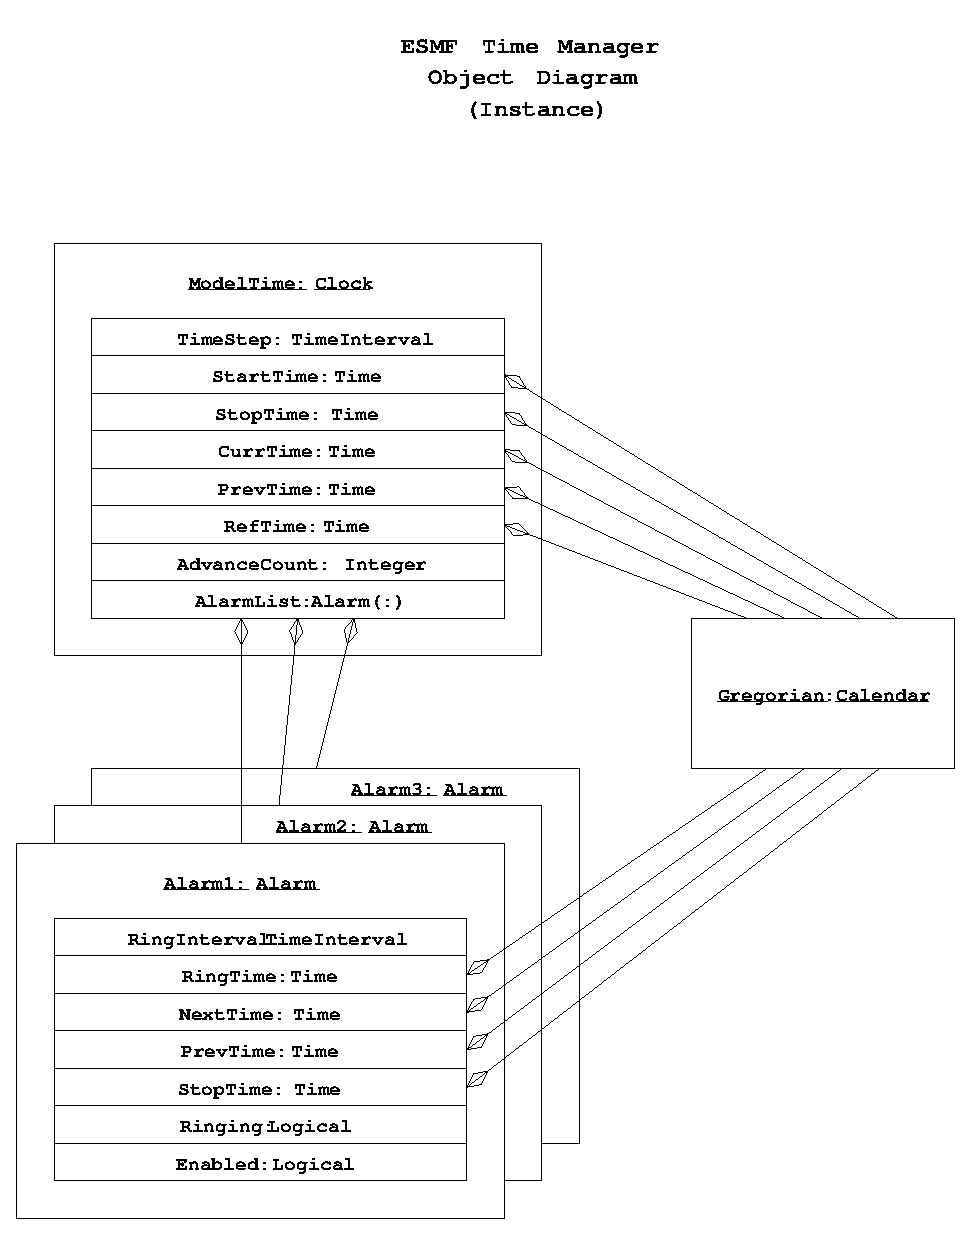
\includegraphics{TimeMgrObject.EPS}
   
Figure 2.  ESMF Time Manager Object Diagram
   
\end{center}

% $Id: TimeMgr_obj3.tex,v 1.2 2003/02/11 18:58:56 eschwab Exp $

%\section{Object Model}

Whereas Figures 1 and 2 are static structure UML diagrams, Figures 3, 4,  and
5 are dynamic behavioral UML diagrams.  Figure 3 shows how timestepping occurs
within an instance of Time Manager.  First, an ESM component invokes the
{\tt Advance()} method on its clock, named {\tt ModelTime} in this example.
In turn, {\tt ModelTime} increments its internal current time, called
{\tt CurrTime}.  A user only needs to know how to create a clock and invoke
its {\tt Advance()} method.  The implementation detail of actually performing
the increment is hidden from the user as it is encapsulated within the Time
Manager clock.

\begin{center}
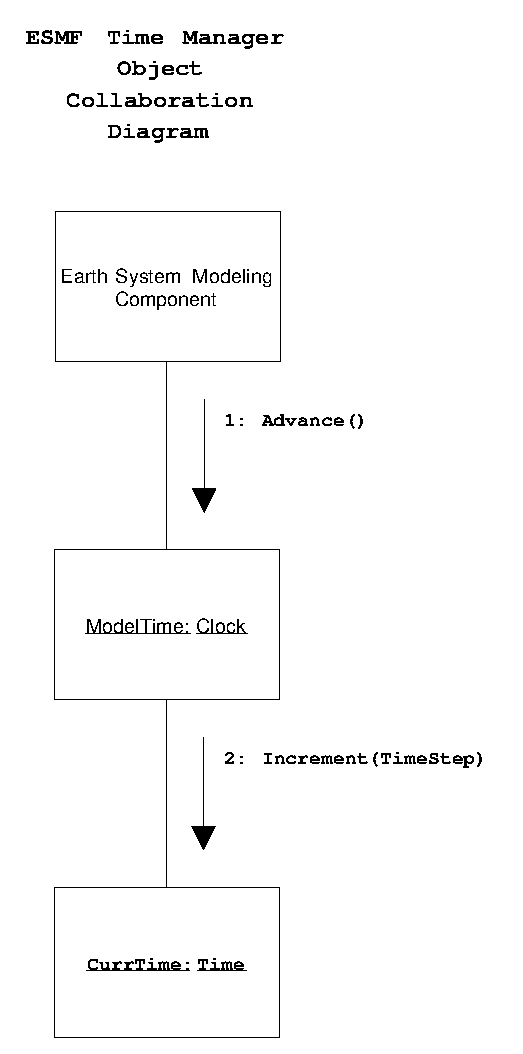
\includegraphics{TimeMgrOCD1.EPS}
   
Figure 3.  ESMF Time Manager Increment Model Time Scenario
   
\end{center}

% $Id: TimeMgr_obj4.tex,v 1.1 2002/08/18 22:43:36 eschwab Exp $

%\section{Object Model}

In Time Manager, all times are internally represented and operated on as
integer seconds and rational integer fractional seconds.  Specific date and
time formats are available to the user at the interface level, where
conversions are performed.  So the user gets/sets Time Manager's TimeIntervals
and TimeInstants in familiar units of year, month, day, hour, minutes,
seconds, and sub-seconds in their various required combinations.  Figure 4
shows an example of a user's ESM component quering its clock for the current
time in (YR, MM, DD, H, M, S) format.  First the model invokes the
Get\_YR\_MM\_DD\_H\_M\_S() method on its clock's current time, CurrTime.  Next,
internally (transparent to the user), CurrTime invokes the ConvertToDate()
method on its associated calendar, Gregorian.  Gregorian, in turn, performs
the requisite conversion of CurrTime's internal representation of time (integer
seconds and fractional seconds) to a Gregorian date.  Note that the calendar
object is a single instance shared among all TimeInstants, as previously shown
in Figures 1 and 2.

\begin{center}
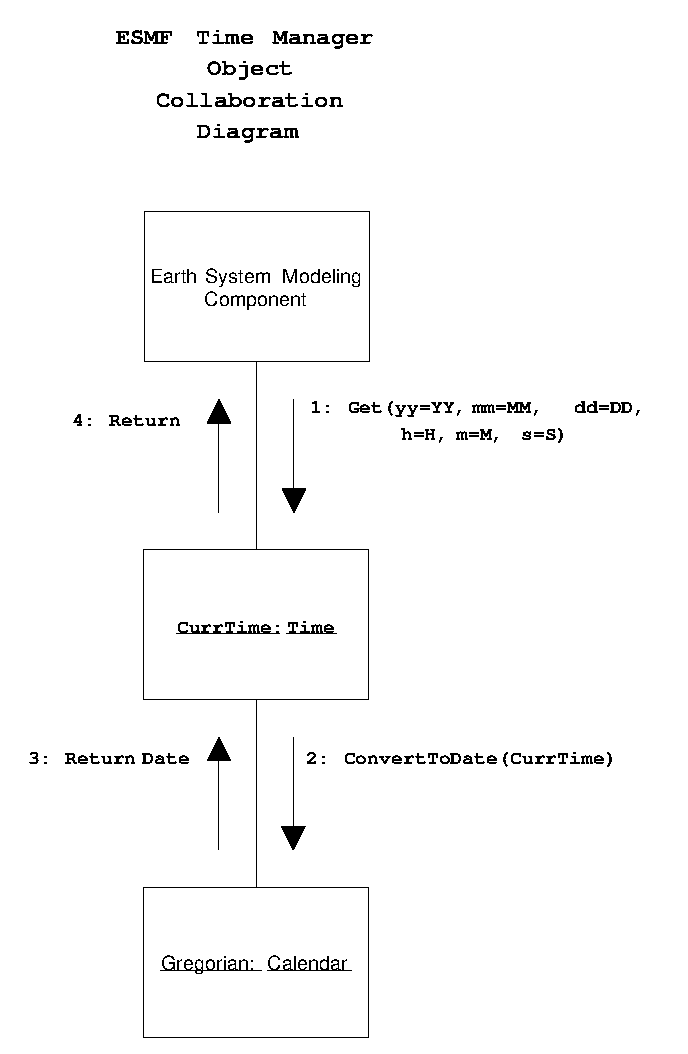
\includegraphics{TimeMgrOCD2.EPS}
   
Figure 4.  ESMF Time Manager Convert to Date Scenario
   
\end{center}

% $Id: TimeMgr_obj5.tex,v 1.1 2002/08/18 22:43:36 eschwab Exp $

%\section{Object Model}

In Figure 5, we see how a ESM component's clock checks its alarms.  After
the clock's current time is incremented (Model time stepped), the clock checks
all its alarms to see if its time for them to start or stop ringing.  All the
user needs to know is how to initialize the alarms and time step the clock;
the alarm checking happens internally "under the hood."
   
\begin{center}
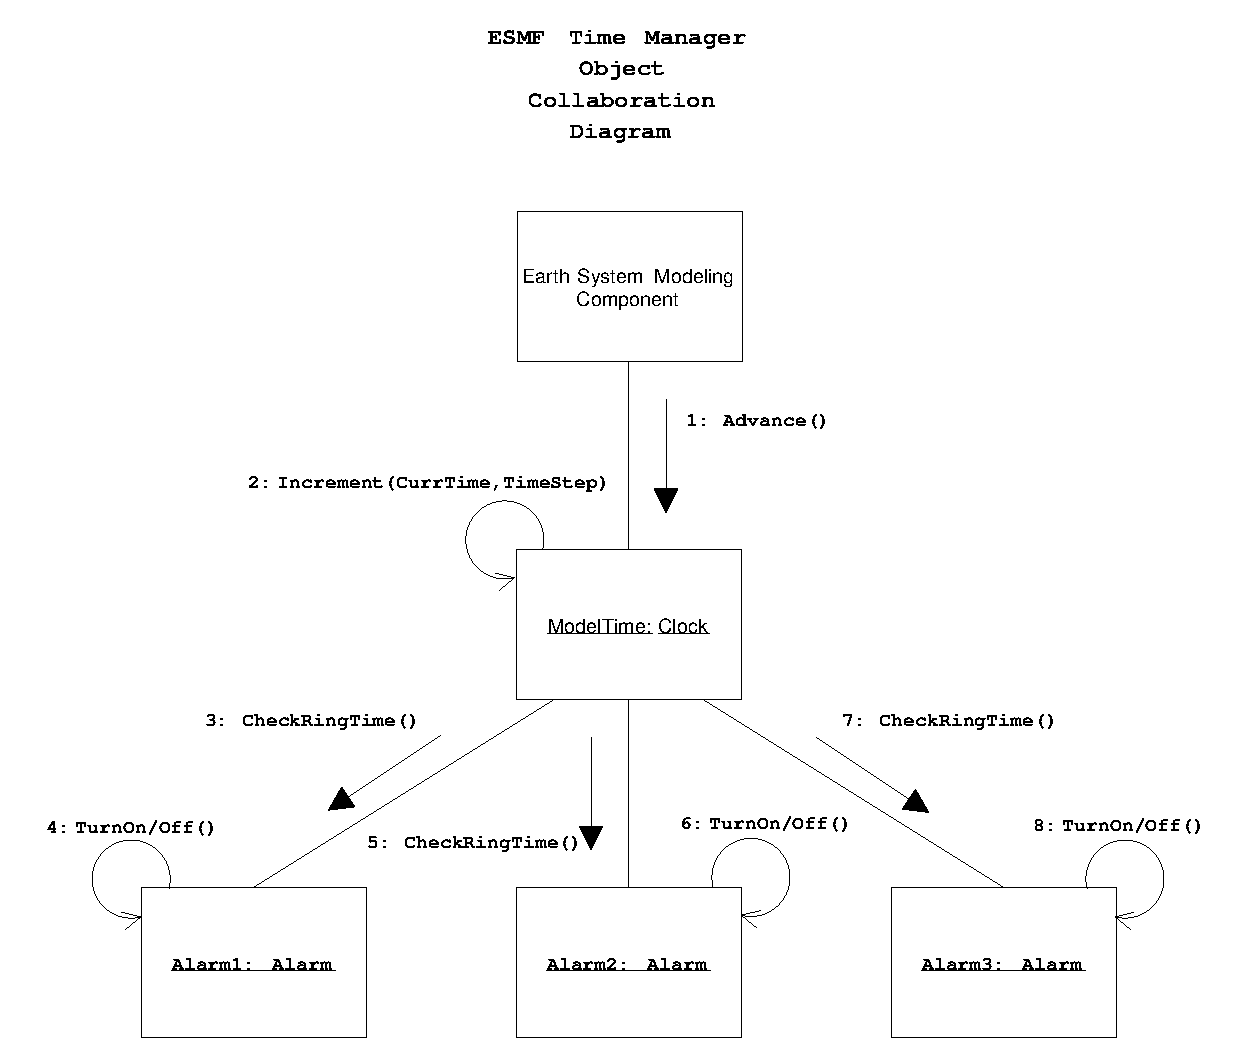
\includegraphics{TimeMgrOCD3.EPS}
   
Figure 5.  ESMF Time Manager Check Alarms Scenario
   
\end{center}


\section{Global Parameters and Definitions}
% $Id: TimeMgr_param.tex,v 1.1 2002/08/18 22:43:36 eschwab Exp $

Platform-independent specification of 64-bit and 32-bit integers are done via
compile-time constants in F90 and C++ as follows:

F90:
\begin{verbatim}
    module ESMF_TypesMod
        integer, parameter :: int64 = selected_int_kind(18) ! 18 decimal digits
        integer, parameter :: int32 = selected_int_kind(9)  ! 9  decimal digits
    end module ESMF_TypesMod
\end{verbatim}

C++:
\begin{verbatim}
#ifdef LIUNX
#define int64  long long	! at least 64 bits
#define int32  long
#elif defined(IRIX64)
#define int64  long			! at least 64 bits
#define int32  long
.
.
.
#endif
\end{verbatim}


% ----------
% Time Class
% ----------

\section{Time Class Design}

\subsection{Description}
% $Id: time_desc.tex,v 1.1 2002/08/18 22:43:37 eschwab Exp $

The Time class is a base class which encapulates the core representation and
functionality of time for time intervals and time instances.


\subsection{Design}
% $Id: time_design.tex,v 1.1 2002/08/18 22:43:37 eschwab Exp $

The Time class is designed with a minimum number of elements to represent
any required time.  The design is based on the idea used in the real-time
POSIX 1003.1b-1993 standard.  That is, to represent time simply as a pair of
integers: one for seconds (whole) and one for nanoseconds (fractional).
These can then be converted at the interface level to any desired format.

For ESMF, this idea is modified and extended, in order to handle the
requirements for a large time range (> 200,000 years) and to exactly
represent any rational fraction, not just nanoseconds.  To handle the
large time range, a 64-bit or greater integer is used for whole seconds.
Any rational fractional second is expressed using two additional integers:
a numerator and a denominator.  Both the whole seconds and fractional numerator
are signed to handle negative time intervals and instants.  The fractional
seconds element (numerator) is \htmlref{normalized}{glos:Normalized} (bounded)
with respect to whole seconds. If the numerator becomes greater than or equal
to the denominator, the whole seconds is incremented accordingly and the
numerator is reset to the remainder.  Conversions are performed upon demand
by interface methods within the derived classes TimeInterval and TimeInstant.
This is done because different applications require different representations
of time intervals and time instances.

The Time class defines increment and decrement methods for basic time
interval calculations between time instants.  It is done here rather than in
the calendar class because it can be done with simple arithmetic that is
calendar-independent.  Upon demand by a user, the results are converted to
user-units via methods in the derived classes TimeInterval and TimeInstant
and the associated Calendar class.

Comparison methods are also defined in the Time class.  These perform
equality/inequality, less than, and greater than comparisons between any two
TimeIntervals or TimeInstants.  These methods capture the common comparison
logic between TimeIntervals and TimeInstants and hence are defined here for
sharing.

The Time class is only a base class not to be instantiated by any application.
It is only used by the derived classes TimeInterval and TimeInstant.


\subsubsection{Class Definition}
% $Id: time_def.tex,v 1.1 2002/08/18 22:43:37 eschwab Exp $
\begin{verbatim}
        type ESMF_Time
            private
            sequence
                integer(int64) :: S     ! whole seconds
                integer(int32) :: Sn    ! fractional seconds, numerator
                integer(int32) :: Sd    ! fractional seconds, denominator
        end type
\end{verbatim}


\subsubsection{Restrictions}
% $Id: time_rest.tex,v 1.1 2002/08/18 22:43:37 eschwab Exp $

The limits on range and resolution of time representation are based on the
64-bit and 32-bit integer types used.  For seconds, a signed 64-bit integer
will have a range of +/- 2\^63-1, or +/- 9223372036854775807.  This corresponds
to a range of +/- (2\^63-1)/(86400 * 365.25) or +/- 292,271,023,045 years, or
about 6 orders of magnitude greater than the required +/- 200,000 years!

For fractional seconds, a signed 32-bit integer will handle a resolution of
+/- 2\^31-1, or +/- 2,147,483,647 parts of a second, which is about twice
that of the required nanosecond resolution.


\section{Time Class F90 Interface}

\subsection{Use and Examples}
% $Id: time_fex.tex,v 1.1 2002/08/18 22:43:37 eschwab Exp $

The Time class is not intended for users; it is only used internally as a base
class for TimeInterval and TimeInstant.  The F90 definition for
TimeInstant is as follows:

\begin{verbatim}
        use ESMF_TimeMod

        type ESMF_TimeInstant
            private
            sequence
                type(ESMF_Time) :: time		! <== "inherits" base class
                integer :: calendar
                integer :: timezone
        end type
\end{verbatim}


\subsection{Parameters and Definitions}
%\input{time_fparam}

%\subsection{Class API}
\input{time_fapi}

\section{Time Class C++ Interface}

\subsection{Use and Examples}
% $Id: time_ccex.tex,v 1.1 2002/08/18 22:43:37 eschwab Exp $

The Time class is not intended for users; it is only used internally as a base
class for TimeInterval and TimeInstant.  The C++ definition for
TimeInstant are as follows:

\begin{verbatim}
class ESMC_TimeInstant : public ESMC_Time   // <== inherits base class
{
  private:

    ESMC_Calendar *Calendar;    // associated calendar
    int Timezone;               // Offset from GMT
};
\end{verbatim}


\subsection{Parameters and Definitions}
%\input{time_ccparam}

%\subsection{Class API}
\input{time_ccapi}

% -------------------
% Time Interval Class
% -------------------

\section{Time Interval Class Design}

\subsection{Description}
% $Id: time_interval_desc.tex,v 1.1 2002/08/18 22:43:37 eschwab Exp $

A TimeInterval inherits from the Time base class and is designed to represent
time deltas which are independent of any calendar.


\subsection{Design}
% $Id: time_interval_design.tex,v 1.1 2002/08/18 22:43:37 eschwab Exp $

TimeInterval inherits from the base class Time.  As such, it gains the core
representation of time as well as its associated methods.   TimeInterval
further specializes Time by adding shortcut methods to set and get a
TimeInterval in natural way with appropriate unit combinations, as per the
requirements.  The largest unit of time for a TimeInterval is a day, so a
TimeInterval is independent of any calendar.  This is in contrast with a
TimeInstant, which is calendar-dependent, since its largest units of time
are months and years.  TimeInterval also defines methods for multiplication
and division of TimeIntervals by integers, reals, fractions and other
TimeIntervals.  TimeInterval does not add any new attributes to Time.


\subsubsection{Class Definition}
% $Id: time_interval_def.tex,v 1.1 2002/08/18 22:43:37 eschwab Exp $
\begin{verbatim}
        type ESMF_TimeInterval 
            private
            sequence
                type(ESMF_Time) :: time
        end type
\end{verbatim}


\subsubsection{Restrictions}
%\input{time_interval_rest}

\section{Time Interval Class F90 Interface}

\subsection{Use and Examples}
$Id: time_interval_fex.tex,v 1.1 2002/08/18 22:43:37 eschwab Exp $

A TimeInterval will typically be used as a timestep for a clock or an alarm
interval.  The following shows how to create and initialize one in F90, based
on the example shown in Figure 2:

\begin{verbatim}
! use the TimeInterval Module
use ESMF_TimeIntervalMod

! create a TimeInterval
type(ESMF_TimeInterval) :: TimeStep

! initialize it to 3 days, 5 hours, 15 minutes, 30 seconds
call ESMF_TimeIntervalInit(TimeStep, D=3, H=5, M=15, S=30)

! pass it to a clock
call ESMF_ClockInit(ModelTime, TimeStep, ...)
\end{verbatim}


\subsection{Parameters and Definitions}
%\input{time_interval_fparam}

%\subsection{Class API}
\input{time_interval_fapi}

\section{Time Interval Class C++ Interface}

\subsection{Use and Examples}
%% $Id: time_interval_ccex.tex,v 1.1 2002/09/20 18:20:15 eschwab Exp $

A TimeInterval will typically be used as a timestep for a clock or an alarm
interval.  The following shows how to create and initialize one in C++, based
on the example shown in Figure 2:

\begin{verbatim}
// use the TimeInterval Class
#include <ESMF_TimeInterval.h>

// instantiate a TimeInterval
ESMC_TimeInterval TimeStep;

// initialize it to 3 days, 5 hours, 15 minutes, 30 seconds
TimeStep.Init("D:H:M:S", 3, 5, 15, 30);

// pass it to a clock
ModelTime.Init(&TimeStep, ...);
\end{verbatim}


\subsection{Parameters and Definitions}
%\input{time_interval_ccparam}

%\subsection{Class API}
\input{time_interval_ccapi}

% ------------------
% Time Instant Class
% ------------------

\section{Time Instant Class Design}

\subsection{Description}
% $Id: time_instant_desc.tex,v 1.1 2002/08/18 22:43:37 eschwab Exp $

A TimeInstant inherits from the Time base class and is designed to represent
a specific point in time which is dependent upon a calendar type.


\subsection{Design}
% $Id: time_instant_design.tex,v 1.1 2002/08/18 22:43:37 eschwab Exp $

TimeInstant inherits from the base class Time.  As such, it gains the core
representation of time as well as its associated methods.   TimeInstant
further specializes Time by adding shortcut methods to set and get a
TimeInstant in a natural way with appropriate unit combinations, as per the
requirements.  A TimeInstant is calendar-dependent, since its largest units
of time are months and years.  TimeInstant also defines special methods for
getting the day of the year, day of the week, middle of the month, and
synchronizing with a real-time clock.  TimeInstant adds its associated
Calendar and local Timezone attributes to Time.


\subsubsection{Class Definition}
% $Id: time_instant_def.tex,v 1.1 2002/08/18 22:43:37 eschwab Exp $
\begin{verbatim}
        type ESMF_TimeInstant
            private
            sequence
                type(ESMF_Time) :: time
                integer :: calendar
                integer :: timezone
        end type
\end{verbatim}


\subsubsection{Restrictions}
%\input{time_instant_rest}

\section{Time Instant Class F90 Interface}

\subsection{Use and Examples}
% $Id: time_instant_fex.tex,v 1.1 2002/08/18 22:43:37 eschwab Exp $

A TimeInstant will typically be used to set the start time in a
clock.  The following shows how to create and initialize one in F90:

\begin{verbatim}
! use the TimeInstant Module
use ESMF_TimeInstantMod

! create a TimeInstant
type(ESMF_TimeInstant) :: StartTime

! initialize it to 8/1/2002, 14:25:45.250, Gregorian calendar
call ESMF_TimeInstantInit(StartTime, YR=2002, MM=8, DD=1, &
                          H=14, M=25, S=45, MS=250, Gregorian)

! pass it to a clock
call ESMF_ClockInit(ModelTime, TimeStep, StartTime, ...)
\end{verbatim}


\subsection{Parameters and Definitions}
%\input{time_instant_fparam}

%\subsection{Class API}
\input{time_instant_fapi}

\section{Time Instant Class C++ Interface}

\subsection{Use and Examples}
%% $Id: time_instant_ccex.tex,v 1.1 2002/09/20 18:20:13 eschwab Exp $

A TimeInstant will typically be used to set the start time in a
clock.  The following shows how to create and initialize one in C++:

\begin{verbatim}
// use the TimeInstant class;
#include <ESMC_TimeInstant.h>

// create a TimeInstant
ESMC_TimeInstant StartTime;

// initialize it to 8/1/2002, 14:25:45.250, Gregorian calendar
StartTime.Init("YR:DD:H:M:S:MS", 2002, 8, 1, 14, 25, 45, 250, Gregorian);

// pass it to a clock
ModelTime.Init(&TimeStep, &StartTime, ...);
\end{verbatim}


\subsection{Parameters and Definitions}
%\input{time_instant_ccparam}

%\subsection{Class API}
\input{time_instant_ccapi}

% --------------
% Calendar Class
% --------------

\section{Calendar Class Design}

\subsection{Description}
% $Id: calendar_desc.tex,v 1.1 2002/08/18 22:43:36 eschwab Exp $

The Calendar class encapsulates the knowledge (attributes and behavior) of all
required calendar types:  Gregorian, Julian, no-leap, 360-day, generic, and
no-calendar.


\subsection{Design}
% $Id: calendar_design.tex,v 1.1 2002/08/18 22:43:36 eschwab Exp $

The Calendar class encapsulates the definition of all required calendar types.
For each calendar type, it contains the number of months per year, the
number of days in each month, the number of seconds in a day, the number of
days per year, and the number of fractional days per year.  This flexible
definition allows future calendars to be defined for any planetary body, not
just Earth. 

The Calendar class defines two methods for converting in both
directions between the core Time class representation and a calendar date.
Calculations of time intervals (deltas) between time instants is done by the
base class Time in the core units of seconds and fractional seconds.  Thus,
a calendar is only needed for converting core time to calendar time and vice
versa.


\subsubsection{Class Definition}
% $Id: calendar_def.tex,v 1.1 2002/08/18 22:43:36 eschwab Exp $
\begin{verbatim}
        integer, parameter :: MonthsPerYear = 12
            
        type ESMF_DaysPerYear
            private
            sequence
                integer :: D    ! whole days per year
                integer :: Dn   ! fractional days per year numerator
                integer :: Dd   ! fractional days per year denominator
        end type

        type ESMF_Calendar
            private
            sequence
                integer :: Type
                integer, dimension(MonthsPerYear) :: DaysPerMonth 
                integer :: SecondsPerDay
                type(ESMF_DaysPerYear) :: DaysPerYear
        end type
\end{verbatim}


\subsubsection{Restrictions}
% $Id: calendar_rest.tex,v 1.1 2002/08/18 22:43:36 eschwab Exp $

Due to the requirement of only Earth modeling and the requirement for no
dynamic memory allocation, the number of months per year is hard-coded
at 12.  However, for easy modification, this is done via an F90 parameter
and a C++ \#define.  See the F90 and C++ "Parameters and Definitions" sections
below.


\section{Calendar Class F90 Interface}

\subsection{Use and Examples}
% $Id: calendar_fex.tex,v 1.1 2002/08/18 22:43:36 eschwab Exp $

A Calendar will be used as a reference for time instants.
The following shows how to create and initialize one in F90:

\begin{verbatim}
! use the Calendar Module
use ESMF_CalendarMod

! create a Calendar
type(ESMF_Calendar) :: Gregorian

! initialize it to be a Gregorian calendar
call ESMF_CalendarInit(Gregorian, ESMF_GREGORIAN)

! pass it to a time instant
call ESMF_TimeInstantInit(StartTime, ..., Gregorian)
\end{verbatim}


\subsection{Parameters and Definitions}
% $Id: calendar_fparam.tex,v 1.1 2002/08/18 22:43:36 eschwab Exp $

The Calendar class has one parameter which defines the number of months
in a year.  For different planetary bodies, this can be edited and
recompiled.

        integer, parameter :: MonthsPerYear = 12

If required, a future enhancement possibility would be to pass this as an
argument to the CalendarInit() method.  The advantage would be no source
code change required, but the disadvantage would be that it requires
dynamic memory allocation, which the requirements document disallows.


%\subsection{Class API}
\input{calendar_fapi}

\section{Calendar Class C++ Interface}

\subsection{Use and Examples}
%% $Id: calendar_ccex.tex,v 1.1 2002/09/20 18:20:11 eschwab Exp $

A Calendar will be used as a reference for time instants.
The following shows how to create and initialize one in C++:

\begin{verbatim}
// use the Calendar class
#include <ESMC_Calendar.h>

// create a Calendar
ESMC_Calendar Gregorian;

// initialize it to be a Gregorian calendar
Gregorian.Init(ESMC_GREGORIAN);

// pass it to a time instant
StartTime.Init(..., Gregorian);
\end{verbatim}


\subsection{Parameters and Definitions}
% $Id: calendar_ccparam.tex,v 1.1 2002/08/18 22:43:36 eschwab Exp $

The Calendar class has one parameter which defines the number of months
in a year.  For different planetary bodies, this can be edited and
recompiled.

        \#define MonthsPerYear 12

If required, a future enhancement possibility would be to pass this as an
argument to the CalendarInit() method.  The advantage would be no source
code change required, but the disadvantage would be that it requires
dynamic memory allocation, which the requirements document disallows.


%\subsection{Class API}
\input{calendar_ccapi}

% -----------
% Clock Class
% -----------

\section{Clock Class Design}

\subsection{Description}
% $Id: clock_desc.tex,v 1.1 2002/08/18 22:43:36 eschwab Exp $

The clock class encapsulates the essential ESM component requirement of
tracking and time-stepping model time.  It also checks associated alarms to
trigger their ringing state.


\subsection{Design}
% $Id: clock_design.tex,v 1.1 2002/08/18 22:43:36 eschwab Exp $

The Clock class contains TimeInstants and a TimeInterval to track and time
step model time.  For tracking, TimeInstants are instantiated for the
current time, stop time, start time, reference time, and previous time. For
time stepping, a single TimeInterval is instantiated.  There is also an
integer counter for keeping track of the number of timesteps, and an array
of associated alarms.  Methods are defined for advancing the clock (perform
a time step), checking if the stop time is reached, synchronizing with a
real-time clock, and getting values of the class attributes defined above.
After performing the time step, the advance method will iterate over the
alarm list and return a list of any active alarms.


\subsubsection{Class Definition}
% $Id: clock_def.tex,v 1.1 2002/08/18 22:43:36 eschwab Exp $
\begin{verbatim}
        type ESMF_Clock
            private
            sequence
                type(ESMF_TimeInterval) :: TimeStep
                type(ESMF_TimeInstant)  :: StartTime
                type(ESMF_TimeInstant)  :: StopTime
                type(ESMF_TimeInstant)  :: RefTime
                type(ESMF_TimeInstant)  :: CurrTime
                type(ESMF_TimeInstant)  :: PrevTime
                integer(int32) :: AdvanceCount
                type(ESMF_Alarm), dimension(10) :: AlarmList
                integer :: ClockMutex
        end type
\end{verbatim}


\subsubsection{Restrictions}
% $Id: clock_rest.tex,v 1.1 2002/08/18 22:43:36 eschwab Exp $

The maximum number of alarms that can be associated with a clock is hard-coded
at 10.  This is done via a F90 parameter and a C++ \#define for ease of
modification.  See the F90 and C++ "Parameters and Definitions" sections below.
If needed, this can be changed in a future release to a dynamic value passed
in during runtime initialization.  But the requirement for no dynamic memory
allocation would have to be relaxed.


\section{Clock Class F90 Interface}

\subsection{Use and Examples}
% $Id: clock_fex.tex,v 1.1 2002/08/18 22:43:36 eschwab Exp $

A Clock is the centerpiece of the Time Manager library, used to track time
in an ESM component.  The following shows how to create and initialize one
in F90, based on the example shown in Figure 2:

\begin{verbatim}
! use the Clock Module
use ESMF_ClockMod

! create a Clock
type(ESMF_Clock) :: ModelTime

! create and initialize a calendar
type(ESMF_Calendar) :: Gregorian
call ESMF_CalendarInit(Gregorian, GREGORIAN)

! create and initialize clock time intervals and instants
type(ESMF_TimeInterval) :: TimeStep
type(ESMF_TimeInstant) :: StartTime, StopTime, RefTime

call ESMF_TimeIntervalInit(TimeStep, ...)
call ESMF_TimeInstantInit(StartTime, ..., Gregorian)
call ESMF_TimeInstantInit(StopTime, ..., Gregorian)
call ESMF_TimeInstantInit(RefTime, ..., Gregorian)

! initialize the clock
call ESMF_ClockInit(ModelTime, TimeStep, StartTime, StopTime, RefTime)

! start time stepping
call ESMF_ClockAdvance(ModelTime)
\end{verbatim}


\subsection{Parameters and Definitions}
% $Id: clock_fparam.tex,v 1.1 2002/08/18 22:43:36 eschwab Exp $

The Clock class has one parameter limiting the number of alarms that can be
associated with it.  In F90 this is

        integer, parameter :: MAX\_ALARMS = 10

If needed, and the non-dynamic memory requirement is lifted, this could be
changed in a future release to a dynamic value passed in during run-time
initialization.


%\subsection{Class API}
\input{clock_fapi}

\section{Clock Class C++ Interface}

\subsection{Use and Examples}
%% $Id: clock_ccex.tex,v 1.1 2002/09/20 18:20:12 eschwab Exp $

A Clock is the centerpiece of the Time Manager library, used to track time
in an ESM component.  The following shows how to create and initialize one
in C++, based on the example shown in Figure 2:

\begin{verbatim}
// use the Clock Class
#include <ESMC_Clock.h>

// create a Clock
ESMC_Clock ModelTime;

// create and initialize a calendar
ESMC_Calendar Gregorian;
Gregorian.Init(GREGORIAN);

// create and initialize clock time intervals and instants
ESMC_TimeInterval TimeStep;
ESMC_TimeInstant  StartTime, StopTime, RefTime;

TimeStep.Init(...);
StartTime.Init(..., Gregorian);
StopTime.Init(..., Gregorian);
RefTime.Init(..., Gregorian);

// initialize the clock
ModelTime.Init(TimeStep, StartTime, StopTime, RefTime);

// start time stepping
ModelTime.Advance();
\end{verbatim}


\subsection{Parameters and Definitions}
% $Id: clock_ccparam.tex,v 1.1 2002/08/18 22:43:36 eschwab Exp $

The Clock class has one parameter limiting the number of alarms that can be
associated with it.  In C++ this is

        \#define MAX\_ALARMS 10

If needed, and the non-dynamic memory requirement is lifted, this could be
changed in a future release to a dynamic value passed in during run-time
initialization.


%\subsection{Class API}
\input{clock_ccapi}

% -----------
% Alarm Class
% -----------

\section{Alarm Class Design}

\subsection{Description}
% $Id: alarm_desc.tex,v 1.1 2002/08/18 22:43:36 eschwab Exp $

The Alarm class encapsulates the required alarm behavior, triggering its
ringing state on either a one-shot or repeating interval basis.


\subsection{Design}
% $Id: alarm_design.tex,v 1.1 2002/08/18 22:43:36 eschwab Exp $

The Alarm class contains TimeInstants and a TimeInterval to perform one-shot
and interval alarming.  A single TimeInterval holds the alarm interval if
used.  A TimeInstant is defined for the ring time, used for either the one-shot
alarm time or for the next interval alarm time.  TimeInstants are also
defined for next and previous ring times in keeping track of alarm intervals.
A TimeInstant for stop time defines when alarm intervals end.  If a one-shot
alarm is defined, only the ring time attribute is used, the others are not.
To keep track of alarm state, two logical attributes are defined, one for
ringing on/off, and the other for alarm enabled/disabled.  An alarm is 
enabled by default; if disabled by the user, it does not function at all.

The primary method is to check whether it is time to set the ringer, which
is called by the associated clock after performing a time step.  Other methods
are defined for getting the ringing state, turning the ringer on/off,
enabling/disabling the alarm, and getting/setting the time attributes
defined above.


\subsubsection{Class Definition}
% $Id: alarm_def.tex,v 1.1 2002/08/18 22:43:36 eschwab Exp $
\begin{verbatim}
        type ESMF_Alarm
            private
            sequence
                type(ESMF_TimeInterval) :: RingInterval
                type(ESMF_TimeInstant)  :: RingTime
                type(ESMF_TimeInstant)  :: NextRingTime
                type(ESMF_TimeInstant)  :: PrevRingTime
                type(ESMF_TimeInstant)  :: StopTime
                logical :: Ringing
                logical :: Enabled
                integer :: ID
                integer :: AlarmMutex
        end type
\end{verbatim}


\subsubsection{Restrictions}
%\input{alarm_rest}

\section{Alarm Class F90 Interface}

\subsection{Use and Examples}
% $Id: alarm_fex.tex,v 1.1 2002/08/18 22:43:36 eschwab Exp $

A Alarm is used in conjunction with a clock to ring at certain points in time.
The following shows how to create and initialize two in F90, based on the
example shown in Figure 2.  The first is a one-shot and the second is an
interval alarm.

\begin{verbatim}
! use the Alarm Module
use ESMF_AlarmMod

! create two Alarms
type(ESMF_Alarm) :: Alarm1, Alarm2

! Initialize one to be a one-shot
type(ESMF_TimeInstant) :: AlarmTime
call ESMF_TimeInstantInit(AlarmTime, YR=2002, MM=8, DD=30, Gregorian)
call ESMF_AlarmInit(Alarm1, RingTime=AlarmTime)

! Initialize other to ring on an interval
type(ESMF_TimeInterval) :: AlarmInterval
call ESMF_TimeIntervalInit(AlarmInterval, DD=1)
call ESMF_AlarmInit(Alarm2, RingInterval=AlarmInterval)

! Associate alarms with clock
call ESMF_ClockAddAlarm(ModelTime, Alarm1)
call ESMF_ClockAddAlarm(ModelTime, Alarm2)

! time step, clock reports active alarms in RingingAlarms list
call ESMF_ClockAdvance(ModelTime, RingingAlarms)

! process any active alarms
if (RingingAlarms(1) == Alarm1) then

   ! process Alarm1
   call ProcessAlarm1()

else if (RingingAlarms(2) == Alarm2) then

   ! process Alarm2
   call ProcessAlarm2()

   ! after processing alarms, turn off interval alarm to prepare for next
   !   ring time
   ESMF_AlarmTurnOff(Alarm2)

end if
\end{verbatim}


\subsection{Parameters and Definitions}
%\input{alarm_fparam}

%\subsection{Class API}
\input{alarm_fapi}

\section{Alarm C++ Interface}

\subsection{Use and Examples}
%% $Id: alarm_ccex.tex,v 1.1 2002/09/20 18:20:10 eschwab Exp $

A Alarm is used in conjunction with a clock to ring at certain points in time.
The following shows how to create and initialize two in C++, based on the
example shown in Figure 2.  The first is a one-shot and the second is an
interval alarm.

\begin{verbatim}
// use the Alarm class
#include <ESMC_Alarm.h>

// create two Alarms
ESMC_Alarm Alarm1, Alarm2;

// Initialize one to be a one-shot
ESMC_TimeInstant AlarmTime;
AlarmTime.Init("YR:MM:DD", 2002, 8, 30, Gregorian);
Alarm1.Init(NULL, &AlarmTime, NULL, true);

// Initialize other to ring on an interval
ESMC_TimeInterval AlarmInterval;
AlarmInterval.Init("DD", 1);
Alarm2.Init(&AlarmInterval, NULL, NULL, true);

// Associate alarms with clock
ModelTime.AddAlarm(&Alarm1);
ModelTime.AddAlarm(&Alarm2);

// time step, clock reports active alarms in RingingAlarms list
ESMC_Alarm RingingAlarms[2];
ModelTime.Advance(RingingAlarms);

// process any active alarms
if (RingingAlarms[1] == Alarm1)
{
   // process Alarm1
   ProcessAlarm1();
}
else if (RingingAlarms[2] == Alarm2)
{
   // process Alarm2
   ProcessAlarm2();

   // after processing alarms, turn off interval alarm to prepare for next
   //   ring time
   Alarm2.TurnOff(Alarm2);
}
\end{verbatim}


\subsection{Parameters and Definitions}
%\input{alarm_ccparam}

%\subsection{Class API}
\input{alarm_ccapi}

\section{Review Status}

\noindent{\bf Design Review} \\

\begin{tabular}{r p{1.3in} p{2in}}
{\bf Review Date:} & <Date> \\ \\
{\bf Reviewers:}   & Reviewer           & <Institution> \\
                   & Reviewer           & <Institution> \\
                   & Reviewer           & <Institution>
\end{tabular}

\section{Glossary}
% $Id: TimeMgr_glos.tex,v 1.1 2002/08/18 22:43:36 eschwab Exp $

% USAGE NOTE:
%
% The first use of a term in the text of a document can be 
% linked to the corresponding glossary item using the item label.
% 
% For example,
%
% Original document text: code must include item1
%
% Linked to glossary:     code must include \htmlref{item1}{glos:item1}
%
% The link will appear in the html version of the document.
% The print version of the document will appear unchanged.

\begin{description}

\item [Normalized] \label{glos:Normalized} To limit the value of a given
time element to the next higher time element used.  For example, if
seconds and days are used, limit seconds to 86400, beyond which days
is incremented.  Similarly, if seconds and hours are used, limit seconds
to 3600.  For fractional seconds, if the numerator becomes >= denominator,
the whole seconds part is incremented and the numerator is reset to the
remainder.

\item [Bounded] \label{glos:Bounded} Synonymous with Normalize.

\end{description}


%\section{Bibliography}
\bibliography{comp} 
\bibliographystyle{plain}
\addcontentsline{toc}{section}{Bibliography}

\end{document}
